\chapter{Time series models}\label{chap8}

\section{Solutions of Exercises}\label{sec81}
\begin{enumerate}[leftmargin=*]
	
	\item Simulate the \textit{dynamic linear model} assuming $X_t\sim N(1, 0.1\sigma^2)$, $w_t\sim N(0, 0.5\sigma^2)$, $\mu_t\sim N(0, \sigma^2)$, $\beta_0=1$, ${B}_0=0.5\sigma^2$, $\sigma^2=0.25$, and ${G}_t=1$, $t=1,\dots,100$. Then, perform the filtering recursion fixing $\Sigma=25\times 0.25$, $\Omega_1=0.5\Sigma$ (high signal-to-noise ratio) and  $\Omega_2=0.1\Sigma$ (low signal-to-noise ratio). Plot and compare the results. 	
	
	\textbf{Answer}
	
	The following code shows how to perform this simulation and perform the filtering recursion using the \textit{dlm} package in \textbf{R}. 
	
	\begin{tcolorbox}[enhanced,width=4.67in,center upper,
		fontupper=\large\bfseries,drop shadow southwest,sharp corners]
		\textit{R code. Simulation: Scenarios signal-to-noise ratio}
		\begin{VF}
			\begin{lstlisting}[language=R]
rm(list = ls()); set.seed(010101)
T <- 100; sig2 <- 0.5^2; r <- 0.5; sigW2 <- sig2*r
x <- rnorm(T, mean = 1, sd = 0.1*sig2^0.5) 
e <- rnorm(T, mean = 0, sd = sig2^0.5)
w <- rnorm(T, mean = 0, sd = sigW2^0.5)
K <- 1 
Bt <- matrix(NA, T, K); Bt[1] <- 1
yt <- rep(NA, T) 
yt[1] <- x[1]*Bt[1] + e[1]
for(t in 1:T){
	if(t == 1){
		Bt[t,] <- w[t]
	}else{
		Bt[t,] <- Bt[t-1,] + w[t]
	}
	yt[t] <- x[t]%*%Bt[t,] + e[t]
}
# State spece model
ModelReg <- function(par){
	Mod <- dlm::dlmModReg(x, dV = exp(par[1]), dW = exp(par[2]), m0 = rep(1, K),
	C0 = sigW2*diag(K), addInt = FALSE)
	return(Mod)
}
sig2New <- sig2*25
RegFilter1 <- dlm::dlmFilter(yt, ModelReg(c(sig2New, sig2New*0.5)))
ytfil1 <- RegFilter1[["m"]][-1]
RegFilter2 <- dlm::dlmFilter(yt, ModelReg(c(sig2New, sig2New*0.1)))
ytfil2 <- RegFilter2[["m"]][-1]
Time <- 1:T
df1 <- as.data.frame(cbind(Time,yt, ytfil1, ytfil2))
library(ggplot2)
ggplot(df1, aes(x=Time)) +
geom_line(aes(y=yt), colour="black", linewidth=1, linetype=1) +
geom_line(aes(y=ytfil1), colour="green", linewidth=1, alpha=0.9, linetype=2) +
geom_line(aes(y=ytfil2), color="blue", linewidth=1, alpha=0.9, linetype=3)\end{lstlisting}
		\end{VF}
	\end{tcolorbox}

\begin{figure}[!h]
	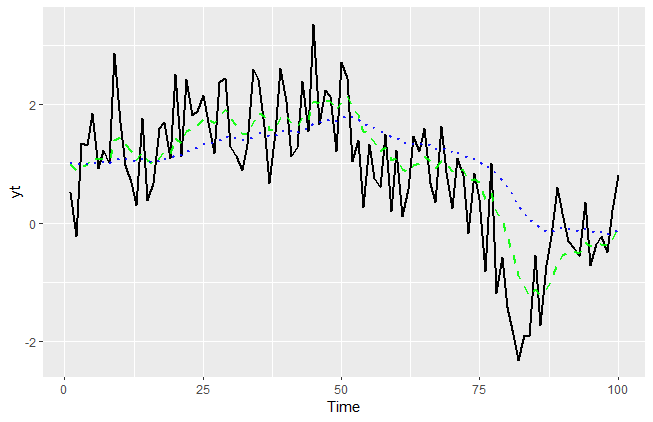
\includegraphics[width=340pt, height=200pt]{Chapters/chapter8/figures/SignaToNoise.png}
	\caption[List of figure caption goes here]{Signal-to-noise ratio: Dynamic linear model.}\label{fig1}
\end{figure} 

Figure \ref{fig1} shows the results of the filtering recursion. We see in this figure that the filtered recursion associated with the high signal-to-noise ratio (green dashed line) follows closer the data than the low signal-to-noise ratio scenario (blue dotted line). We see that the latter is smoother as it gives more weight to the prior mean, which takes into account historical information.

\item Simulate the \textit{dynamic linear model} $y_t=\beta_t x_t + \mu_t$, $\beta_t=\beta_{t-1}+w_t$, where $x_t\sim N(1, 0.1\sigma^2)$, $w_t\sim N(0, 0.5\sigma^2)$, $\mu_t\sim N(0, \sigma^2)$, $\beta_0=0$, $B_0=0.5\sigma^2$, and $\sigma^2=1$, $t=1,\dots,100$. Perform the filtering and smoothing recursions from scratch. 	

\textbf{Answer}

The following code shows how to perform this simulation and perform the filtering recursion from scratch in \textbf{R}. 

\begin{tcolorbox}[enhanced,width=4.67in,center upper,
	fontupper=\large\bfseries,drop shadow southwest,sharp corners]
	\textit{R code. Simulation: Filtering and smoothing recursions from scratch}
	\begin{VF}
		\begin{lstlisting}[language=R]
rm(list = ls()); set.seed(010101)
T <- 100; sig2 <- 1; r <- 0.5; sigW2 <- sig2*r
xt <- rnorm(T, mean = 1, sd = 0.1*sig2^0.5) 
e <- rnorm(T, mean = 0, sd = sig2^0.5)
w <- rnorm(T, mean = 0, sd = sigW2^0.5)
K <- 1; Bt <- matrix(NA, T, K); Bt[1] <- 0
yt <- rep(NA, T)
for(t in 1:T){
	if(t == 1){
		Bt[t,] <- w[t]
	}else{
		Bt[t,] <- Bt[t-1,] + w[t]
	}
	yt[t] <- xt[t]%*%Bt[t,] + e[t]
}
# Filtering
KFR <- function(y, x, b1, B1, Omega, sig2){
	e <- as.numeric(y - t(x)%*%b1) # Error
	R <- B1 + Omega
	q <- as.numeric(t(x)%*%R%*%x + sig2)
	K <- (R%*%x)/q
	bt <- b1 + K*e
	Bt <- R - R%*%x%*%t(x)%*%R/q
	Result <- list(bt = bt, Bt = Bt) 
	return(Result)
}
KFresb <- list(); KFresB <- list()
b0 <- 0; B0 <- sigW2
for(t in 1:T){
	KFrest <- KFR(y = yt[t], x = xt[t], b1 = b0, B1 = B0, Omega = sigW2, sig2 = sig2)
	b0 <- KFrest[["bt"]]; B0 <- KFrest[["Bt"]]
	KFresb[[t]] <- b0; KFresB[[t]] <- B0 
}
ModelReg <- function(par){
	Mod <- dlm::dlmModReg(xt, dV = exp(par[1]), dW = exp(par[2]), m0 = rep(0, K),
	C0 = sigW2*diag(K), addInt = FALSE)
	return(Mod)
}
RegFilter1 <- dlm::dlmFilter(yt, ModelReg(c(sig2, sigW2)))
plot(Bt, type = "l")
lines(unlist(KFresb), type = "l", col = "red")
lines(RegFilter1[["m"]][-1], type = "l", col = "blue")
\end{lstlisting}
	\end{VF}
\end{tcolorbox}

\begin{tcolorbox}[enhanced,width=4.67in,center upper,
	fontupper=\large\bfseries,drop shadow southwest,sharp corners]
	\textit{R code. Simulation: Filtering and smoothing recursions from scratch}
	\begin{VF}
		\begin{lstlisting}[language=R]
# Smoothing 
BSR <- function(b, B, slead, Slead, Omega){
	b = bfilter[t]; B = Bfilter[t]; slead = slead; Slead = slead; Omega = sigW2
	R1 <- B + Omega
	s <- b + B%*%solve(R1)%*%(slead - b)
	S <- B - B%*%solve(R1)%*%(R1 - Slead)%*%solve(R1)%*%B
	Result <- list(st = s, St = S) 
	return(Result)
}
bfilter <- unlist(KFresb); Bfilter <- unlist(KFresB)
slead <- bfilter[T]; Slead <- Bfilter[T]
smooth <- rep(slead, T); Smooth <- rep(Slead, T);  
for(t in (T-1):1){
	BSRrest <- BSR(b = bfilter[t], B = Bfilter[t], slead = slead, Slead = Slead, Omega = sigW2)
	slead <- BSRrest[["st"]]; Slead <- BSRrest[["st"]]
	smooth[t] <- slead
}
RegSmoth <- dlm::dlmSmooth(yt, ModelReg(c(sig2, sigW2)))
VarSmooth <- dlm::dlmSvd2var(u = RegSmoth[["U.S"]], RegSmoth[["D.S"]])
SDVarSmoothB2 <- sapply(2:(T+1), function(t){VarSmooth[[t]][K,K]^0.5}) 
plot(Bt, type = "l")
lines(smooth, type = "l", col = "orange")
lines(RegSmoth[["s"]][-1], type = "l", col = "green")
\end{lstlisting}
	\end{VF}
\end{tcolorbox}

	\item Show that in the $AR(2)$ stationary process, $y_t=\mu+\phi_1y_{t-1}+\phi_2y_{t-2}+e_t$, where $e_t\sim N(0,\sigma^2)$, $\mathbb{E}[y_t]=\frac{\mu}{1-\phi_1-\phi_2}$, and $Var[y_t]=\frac{\sigma^2(1-\phi_2)}{1-\phi_2-\phi_1^2-\phi_1^2\phi_2-\phi_2^2+\phi_2^3}$.
	
	\textbf{Answer}
	
	A necessary condition to achieve second-order stationarity in the $AR(2)$ process is that roots of of the polynomial $1-\phi_1L-\phi_2L^2=0$ lie outside the unit circle. This is achieved if $|\phi_2|<1$, $\phi_1+\phi_2<1$ and $\phi_2-\phi_1<1$.
	
	Let's calculate the expected value:
	\begin{align*}
		\mathbb{E}[y_t]&=\bar{\mu}\\
			&=\mathbb{E}[\mu+\phi_1y_{t-1}+\phi_2y_{t-2}+e_t]\\
			&=\mu+\phi_1\mathbb{E}[y_{t-1}]+\phi_2\mathbb{E}[y_{t-2}]+\mathbb{E}[e_{t}]\\
			&=\mu+\phi_1\bar{\mu}+\phi_2\bar{\mu},
	\end{align*}
then, $\bar{\mu}(1-\phi_1-\phi_2)=\mu$, then, $\mathbb{E}[y_t]=\bar{\mu}=\frac{\mu}{1-\phi_1-\phi_2}$.

See that $y_t=\mu+\phi_1y_{t-1}+\phi_2y_{t-2}+e_t$ implies that $y_t=\bar{\mu}(1-\phi_1-\phi_2)+\phi_1y_{t-1}+\phi_2y_{t-2}+e_t$, which means that $y_t-\bar{\mu}=\phi_1(y_{t-1}-\bar{\mu})+\phi_2(y_{t-2}-\bar{\mu})+e_t$, and setting $z_t=y_t-\bar{\mu}$, we have $z_t=\phi_1z_{t-1}+\phi_2z_{t-2}+e_t$ where $\mathbb{E}[z_t]=0$. Then, we can calculate the variance of $y_t$ using $z_t$, given that both have same variance.  

Let's define $\gamma_s=Cov(z_t,z_{t-s})=\mathbb{E}[z_tz_{t-s}]$, then the Yule-Walker equations are:
\begin{align*}
	\gamma_0&=\phi_1\gamma_1+\phi_2\gamma_2+\sigma^2\\
	\gamma_1&=\phi_1\gamma_0+\phi_2\gamma_1\\
	\gamma_2&=\phi_1\gamma_1+\phi_2\gamma_0.
\end{align*}  
Solving this system of equations for $\gamma_0$, $\gamma_1$ and $\gamma_2$, we find that $\gamma_0=\frac{\sigma^2(1-\phi_2)}{1-\phi_2-\phi_1^2-\phi_1^2\phi_2-\phi_2^2+\phi_2^3}$. 
	

\item Show that the posterior distribution of $\bm{\phi}|\bm{\beta},\sigma^2,\bm{y},\bm{X}$ in the model $y_t=\bm{x}_t^{\top}\bm{\beta}+\mu_t$ where $\phi(L)\mu_t=e_t$ and $e_t\stackrel{iid}{\sim}N(0,\sigma^2)$ is $N(\bm{\phi}_n, \bm{\Phi}_n)\mathbbm{1}[\bm{\phi}\in S_{\bm{\phi}}]$, where $\bm{\Phi}_n=(\bm{\Phi}_0^{-1}+\sigma^{-2}\bm{U}^{\top}\bm{U})$, $\bm{\phi}_n=\bm{\Phi}_n(\bm{\Phi}_0^{-1}\bm{\phi}_0+\sigma^{-2}\bm{U}^{\top}\bm{\mu})$, and $S_{\phi}$ is the stationary region of $\bm{\phi}$.
	
\textbf{Answer}
	
The conditional posterior distribution can be got as follows:
	\begin{align*}
		\pi(\bm{\phi}|\bm{\beta},\sigma^2,\bm{y})&\propto \exp\left\{-\frac{1}{2\sigma^2}(\bm{\mu}-\bm{U}\bm{\phi})^{\top}(\bm{\mu}-\bm{U}\bm{\phi})\right\}\\
		&\times \exp\left\{-\frac{1}{2}(\bm{\phi}-\bm{\phi}_0)^{\top}\bm{\Phi}_0^{-1}(\bm{\phi}-\bm{\phi}_0)\right\}\\
		&\propto\exp\left\{-\frac{1}{2}[\bm{\phi}^{\top}(\sigma^{-2}\bm{U}^{\top}\bm{U}+\bm{\Phi}_0^{-1})\bm{\phi}-2\bm{\phi}^{\top}(\sigma^{-2}\bm{U}^{\top}\bm{\mu}+\bm{\Phi}_0^{-1}\bm{\phi}_0)\right.\\
		&\left.+\bm{\phi}_n^{\top}\bm{\Phi}_n^{-1}\bm{\phi}_n-\bm{\phi}_n^{\top}\bm{\Phi}_n^{-1}\bm{\phi}_n]\right\}\\
		&\propto\exp\left\{-\frac{1}{2}[(\bm{\phi}-\bm{\phi}_n)^{\top}\bm{\Phi}_n^{-1}(\bm{\phi}-\bm{\phi}_n)]\right\}, 
	\end{align*}
where $\bm{\Phi}_n=(\sigma^{-2}\bm{U}^{\top}\bm{U}+\bm{\Phi}_0^{-1})^{-1}$ and $\bm{\phi}_n=\bm{\Phi}_n(\sigma^{-2}\bm{U}^{\top}\bm{\mu}+\bm{\Phi}_0^{-1}\bm{\phi}_0)$. The last expression is the kernel of a multivariate normal distribution with mean $\bm{\phi}_n$ and variance matrix $\bm{\Phi}_n$.   
	
\end{enumerate}